\documentclass[preview]{standalone}
\usepackage{tikz}
\usepackage{fancyvrb}
\usepackage{xcolor}
\usepackage{soul}

\definecolor{lightpink}{rgb}{1.0, 0.71, 0.76}
\definecolor{lightblue}{rgb}{0.68, 0.85, 0.9}
\definecolor{lightgreen}{rgb}{0.56, 0.93, 0.56}
\newcommand{\hlred}[1]{\sethlcolor{lightpink}\hl{#1}}
\newcommand{\hlblue}[1]{\sethlcolor{lightblue}\hl{#1}}
\newcommand{\hlgreen}[1]{\sethlcolor{lightgreen}\hl{#1}}

% \nodehere node_name 
\newcommand{\nodehere}[1]{\tikz{[remember picture] \node[coordinate] (#1) {}; }}
\newcommand{\zseton}[1]{\tikz{[remember picture] \node[circle, fill=red, inner sep=2pt] (#1) {}; }}

%
\newcommand{\hframe}[5]{%
    \coordinate (BF) at (#1);
    \coordinate (JA) at ($ (BF) + (3,-2) $);
    \coordinate (CSB) at ($ (BF) + (0,-0.5) $);
    \coordinate (CSJ) at ($ (BF) + (3,-0.5) $);
    \draw (BF) rectangle (JA);
    \draw (CSB) -- (CSJ) node [above, pos=0.5] (A) {#2} node [below, pos=0.5] (B)
    {\begin{tabular}{c}pc = #3 \\ A = #4\\ S=[#5]\end{tabular}};%
}

\usetikzlibrary{positioning}
\usetikzlibrary{calc}
\usetikzlibrary{decorations.pathmorphing}

\tikzstyle{every picture}+=[remember picture]

\tikzset{snake it/.style={decorate, decoration={snake, segment length=1.5mm, amplitude=0.5mm}}}
\tikzset{
    position/.style args={#1:#2 from #3}{
        at=(#3.#1), anchor=#1+180, shift=(#1:#2)
    }
}

\begin{document}
\begin{minipage}{4\textwidth}
\begin{Verbatim}[commandchars=\\\{\}]
    effect Choose : unit -->> bool;;

    let h = handler
    | \colorbox{blue!30}{val x -> [x]}
    | \colorbox{red!30}{effect (Choose ()) k ->}
        \colorbox{red!30}{(continue k true) @ (continue k false)}
    | \colorbox{purple!30}{finally x -> x}
    ;;
    
    \colorbox{orange!30}{with h handle}
        \colorbox{green!30}{let x = if (perform (Choose ())) then 10 else 20 in}
        \colorbox{green!30}{let y = if (perform (Choose ())) then 5 else 15 in}
        \colorbox{green!30}{x - y}
    ;;
\end{Verbatim}
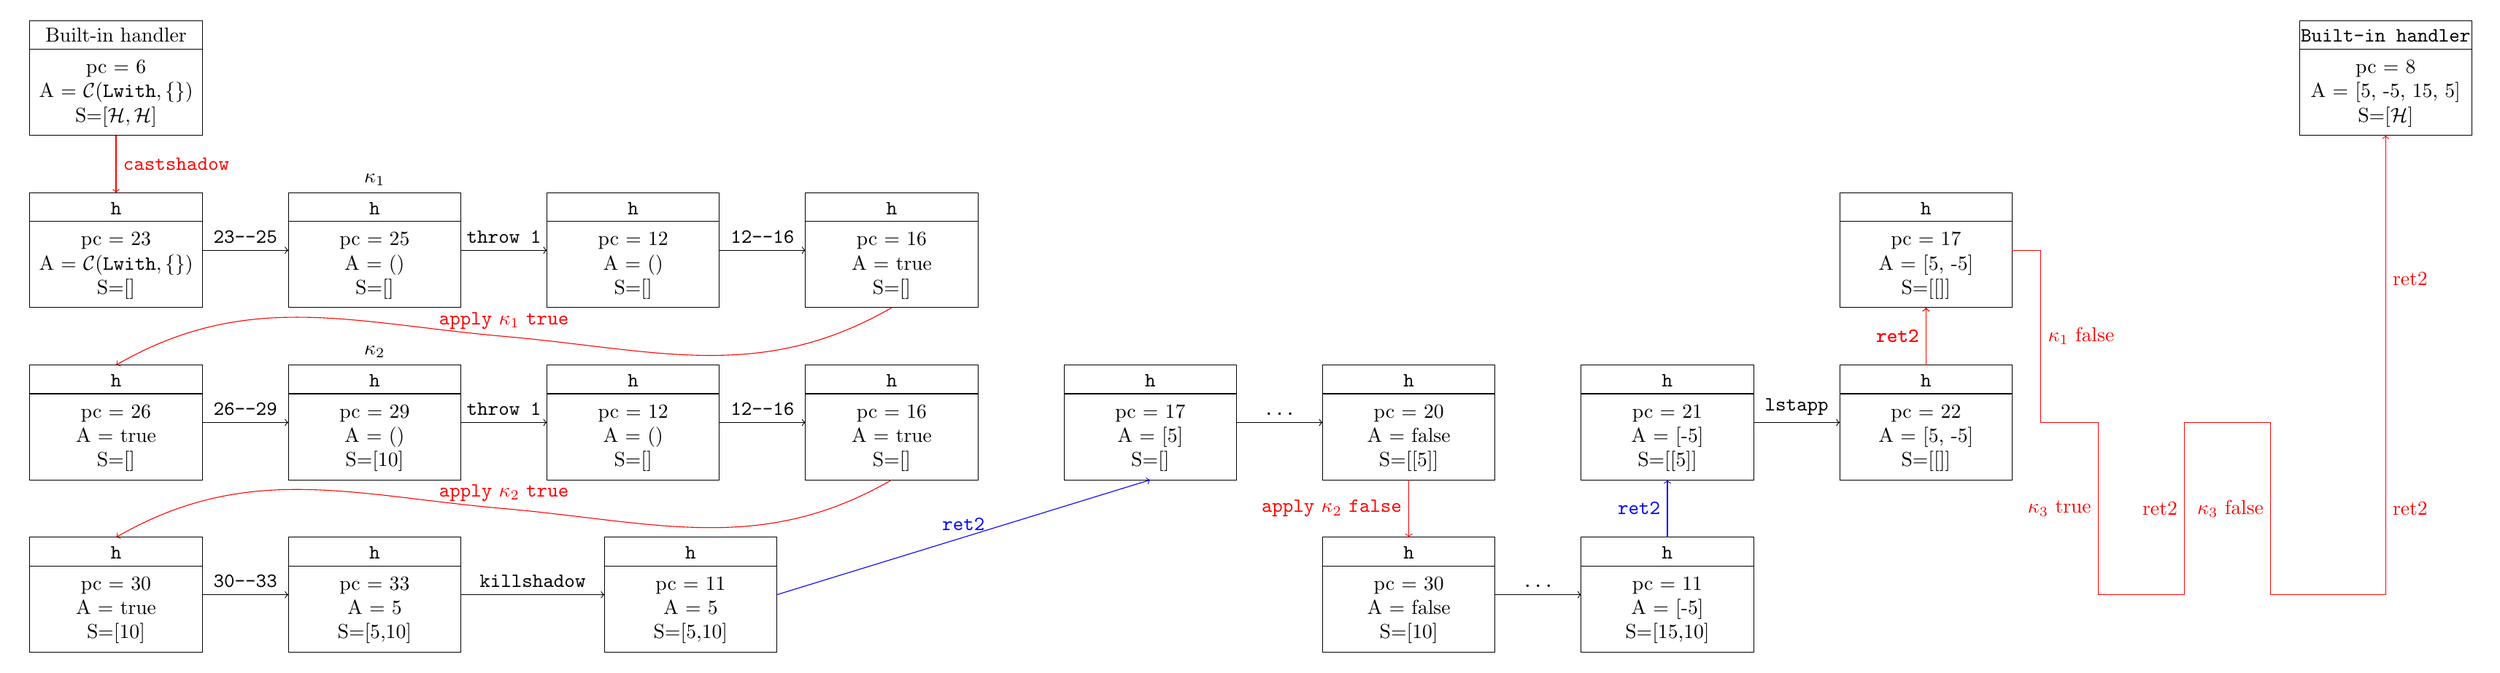
\begin{tikzpicture}
    \hframe{0,0}{Built-in handler}{6}{$\mathcal{C}(\mathtt{Lwith}, \{\})$}{$\mathcal{H},\mathcal{H}$};
    \draw[->, red] (1.5, -2) -- (1.5, -3) node [right, pos=0.5] (C) {\verb|castshadow|};

    \hframe{0,-3}{\texttt{h}}{23}{$\mathcal{C}(\mathtt{Lwith}, \{\})$}{};
    \draw[->] (3, -4) -- (4.5, -4) node [above, pos=0.5] (C) {\verb|23--25|};

    \hframe{4.5,-3}{\texttt{h}}{25}{()}{};
    \draw[->] (7.5, -4) -- (9, -4) node [above, pos=0.5] (C) {\verb|throw 1|};
    \node [above] (kappa1) at (6,-3) {$\kappa_1$};

    \hframe{9,-3}{\texttt{h}}{12}{()}{};
    \draw[->] (12, -4) -- (13.5, -4) node [above, pos=0.5] (C) {\verb|12--16|};
    
    \hframe{13.5,-3}{\texttt{h}}{16}{true}{};
    \draw[->, red] (15,-5) to [in=-5, out=-150] (8.25, -5.5) node [above] (X) {\verb|apply| $\kappa_1$ \verb|true|} to [out=175,in=30] (1.5,-6);
    
    %%%%%%

    \hframe{0,-6}{\texttt{h}}{26}{true}{};
    \draw[->] (3, -7) -- (4.5, -7) node [above, pos=0.5] (C) {\verb|26--29|};
    
    \hframe{4.5,-6}{\texttt{h}}{29}{()}{10};
    \draw[->] (7.5, -7) -- (9, -7) node [above, pos=0.5] (C) {\verb|throw 1|};

    \hframe{9,-6}{\texttt{h}}{12}{()}{};
    \draw[->] (12, -7) -- (13.5, -7) node [above, pos=0.5] (C) {\verb|12--16|};
    \node [above] (kappa1) at (6,-6) {$\kappa_2$};

    \hframe{13.5,-6}{\texttt{h}}{16}{true}{};
    \draw[->, red] (15,-8) to [in=-5, out=-150] (8.25, -8.5) node [above] (X) {\verb|apply| $\kappa_2$ \verb|true|} to [out=175,in=30] (1.5,-9);

    %%%%%%

    \hframe{0,-9}{\texttt{h}}{30}{true}{10};
    \draw[->] (3, -10) -- (4.5, -10) node [above, pos=0.5] (C) {\verb|30--33|};

    \hframe{4.5,-9}{\texttt{h}}{33}{5}{5,10};
    \draw[->] (7.5, -10) -- (10, -10) node [above, pos=0.5] (C) {\verb|killshadow|};
    
    \hframe{10,-9}{\texttt{h}}{11}{5}{5,10};

    %%%%%%

    \hframe{18,-6}{\texttt{h}}{17}{[5]}{};
    \draw[->, blue] [bend right] (13,-10) -- (19.5,-8) node [above, pos=0.5] (Z) {\verb|ret2|};
    
    \hframe{22.5,-6}{\texttt{h}}{20}{false}{[5]};
    \draw[->] (21, -7) -- (22.5, -7) node [above, pos=0.5] (C) {\verb|...|};

    \hframe{22.5,-9}{\texttt{h}}{30}{false}{10};
    \draw[red,->] (24, -8) -- (24, -9) node [left, pos=0.5] (C) {\verb|apply| $\kappa_2$ \verb|false|};

    \hframe{27,-9}{\texttt{h}}{11}{[-5]}{15,10};
    \draw[->] (25.5, -10) -- (27, -10) node [above, pos=0.5] (C) {\verb|...|};

    \hframe{27,-6}{\texttt{h}}{21}{[-5]}{[5]};
    \draw[blue, ->] (28.5, -9) -- (28.5, -8) node [left, pos=0.5] (C) {\verb|ret2|};

    \hframe{31.5,-6}{\texttt{h}}{22}{[5, -5]}{[]};
    \draw[->] (30, -7) -- (31.5, -7) node [above, pos=0.5] (C) {\verb|lstapp|};

    \hframe{31.5,-3}{\texttt{h}}{17}{[5, -5]}{[]};
    \draw[red, ->] (33, -6) -- (33, -5) node [left, pos=0.5] (C) {\verb|ret2|};

    \hframe{39.5,0}{\texttt{Built-in handler}}{8}{[5, -5, 15, 5]}{$\mathcal{H}$};
    \draw[red, ->] (33, -6) -- (33, -5) node [left, pos=0.5] (C) {\verb|ret2|};

    \draw[red, ->] (34.5,-4) -- (35,-4) -- (35,-7) node [right, pos=0.5] (C) {$\kappa_1$ false} --
    (36, -7) -- (36, -10) node [left, pos=0.5] (C) {$\kappa_3$ true} -- (37.5, -10) -- (37.5, -7) node [left, pos=0.5] (C) {ret2} --
    (39, -7) -- 
    (39, -10) node [left, pos=0.5] (C) {$\kappa_3$ false} --
    (41, -10)  --
    (41, -7) node [right, pos=0.5] (C) {ret2} --
    (41, -2) node [right, pos=0.5] (C) {ret2} ;

\end{tikzpicture}
\end{minipage}%
\begin{minipage}{0.8\textwidth}
\begin{Verbatim}[numbers=left, commandchars=\\\{\}]
    SHADEcode:
        makehlosure 0, Lval, Lfin, [(Lchoose, 1)]
        push
        push
        makeclosure Lwith, 0
        \nodehere{cast}\colorbox{orange!30}{castshadow}
        \nodehere{fin}\colorbox{orange!30}{fin} \nodehere{fin2}
        halt \nodehere{halt}
    \colorbox{blue!30}{Lval:}
        \colorbox{blue!30}{makebox 0, 1}
        \colorbox{blue!30}{ret2}
    \colorbox{red!30}{Lchoose:} \nodehere{lchoose}
        \colorbox{red!30}{envacc 0}
        \colorbox{red!30}{push}
        \colorbox{red!30}{const true}
        \colorbox{red!30}{apply}
        \colorbox{red!30}{push}
        \colorbox{red!30}{envacc 0}
        \colorbox{red!30}{const false}
        \colorbox{red!30}{apply}
        \colorbox{red!30}{lstappend}
        \colorbox{red!30}{ret2}
    \nodehere{lwith}\colorbox{green!30}{Lwith:}
        \colorbox{green!30}{const ()}
        \colorbox{green!30}{throw 1}\nodehere{firstthrow}
        \colorbox{green!30}{push}
        \colorbox{green!30}{//...}
        \colorbox{green!30}{const ()}
        \colorbox{green!30}{throw 1}
        \colorbox{green!30}{push}
        \colorbox{green!30}{//...}
        \colorbox{green!30}{subint}
        \colorbox{green!30}{killshadow}
    \colorbox{purple!30}{Lfin:}
        \colorbox{purple!30}{ret}
\end{Verbatim}
\end{minipage}
\end{document}